\documentclass[a4paper]{article}
\usepackage[a4paper,margin=0cm,top=1cm]{geometry}

\usepackage[rgb]{xcolor}
\usepackage{tikz}
\usetikzlibrary{shadings}

\begin{document}
\vspace*{\stretch{1}}
\begin{center}
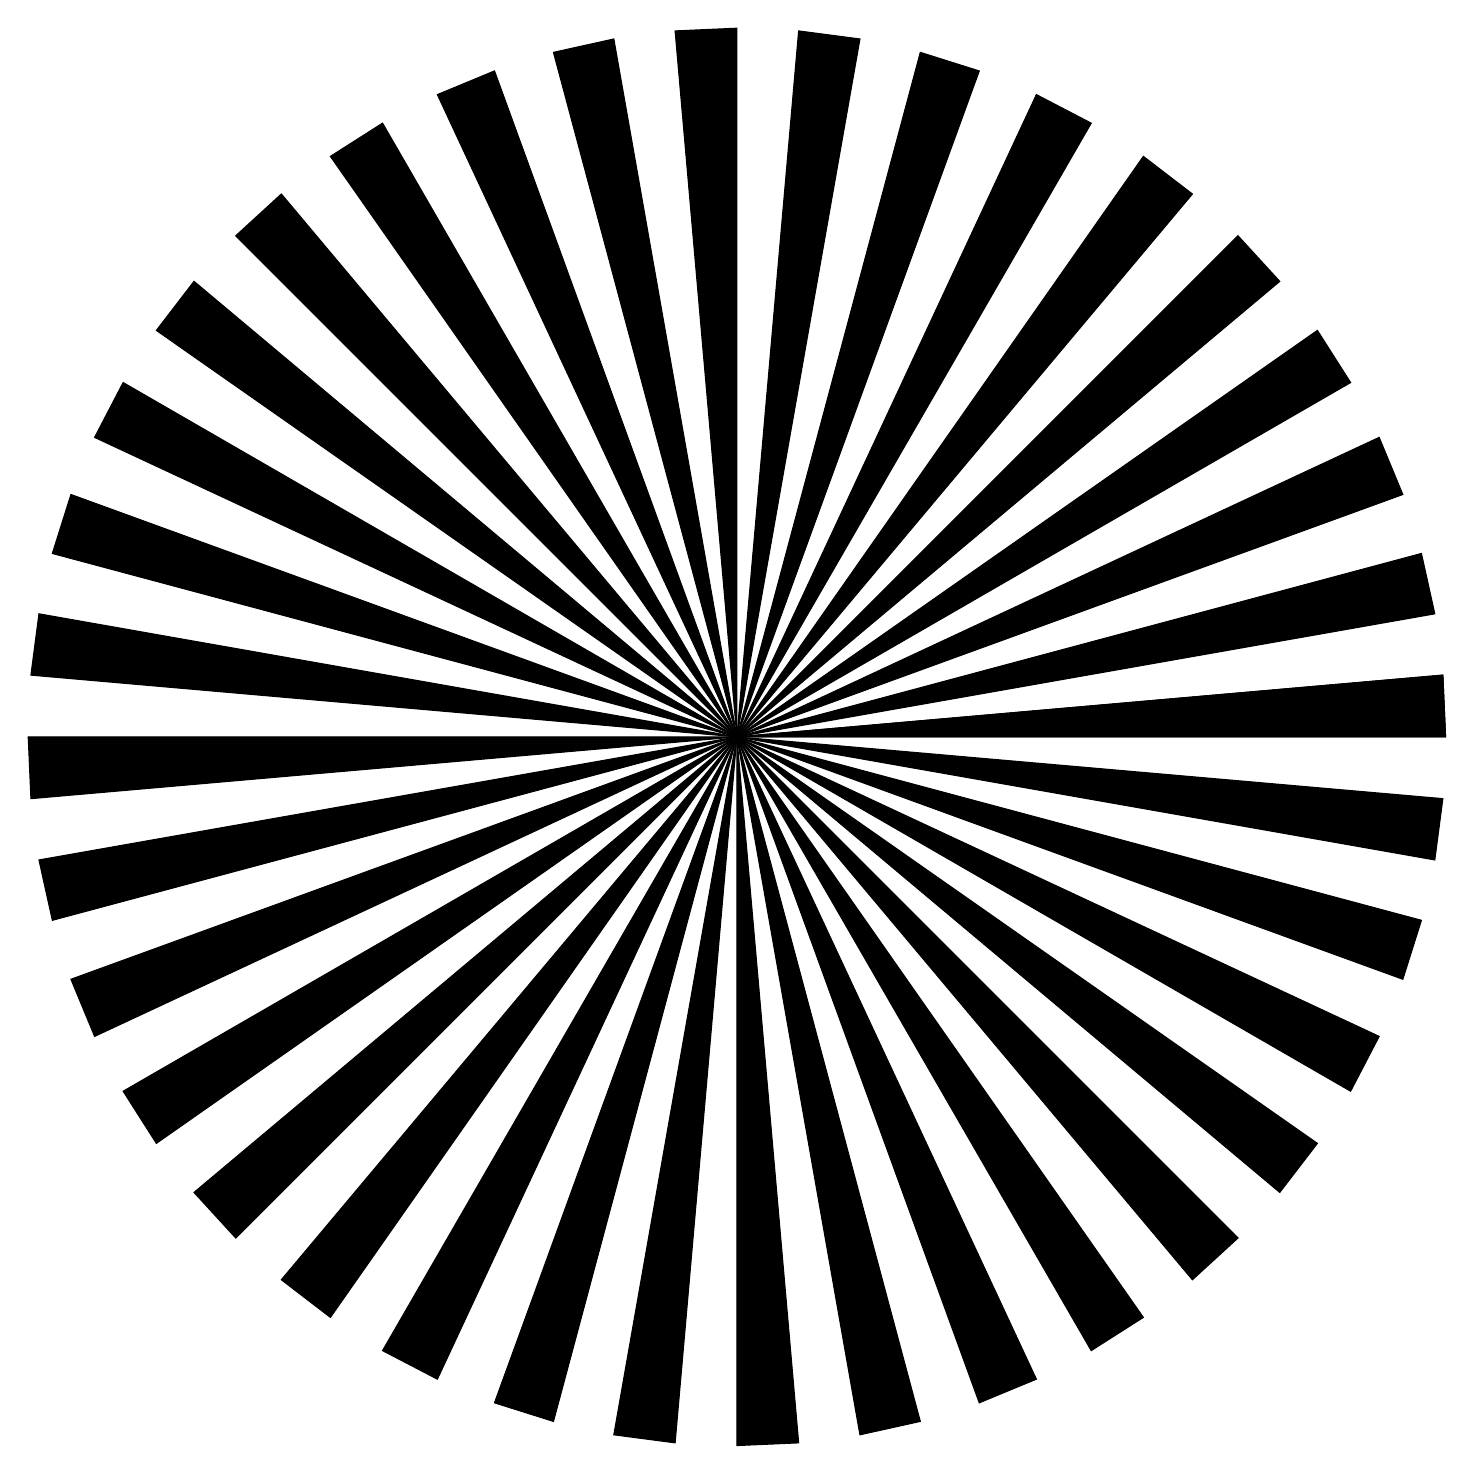
\begin{tikzpicture}[baseline={([yshift=-.8ex]current bounding box.center)}]
    \foreach \angle in {0,10,...,360}
      \draw[fill] (0,0) -- (\angle:9cm) -- (\angle+5:9cm) -- (0,0);
    % \foreach \radius in {1,...,9}
    %   \draw[white,line width=\radius * 0.001 cm] (0,0) circle (\radius cm);
\end{tikzpicture}
\end{center}
\vspace{\stretch{2}}
\end{document}
